% Defense slide (power method): one application of the transfer matrix for BOTH
% boundary states — the right tMPS via E, the left tMPS via E^T — each followed
% by truncation back to chi. Panel (a) reproduces thesis/imgs/apply.tex; panel (b)
% is its mirror for the left state.
\documentclass[tikz,border=3pt]{standalone}
\usepackage{amsmath,amssymb,braket,graphicx}
\usetikzlibrary{arrows.meta}

\definecolor{tnL}{RGB}{243,116,63}
\definecolor{tnR}{RGB}{60,110,150}
\definecolor{tnE}{RGB}{250,200,70}

\newcommand{\DY}{0.72}    % time-site spacing
\newcommand{\LG}{0.42}

\begin{document}
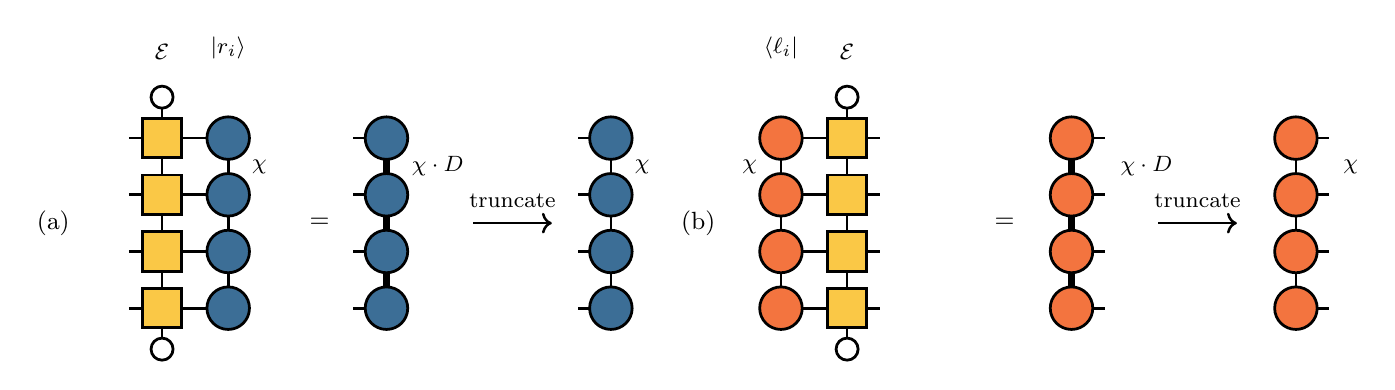
\begin{tikzpicture}[
    bond/.style={draw=black, line width=1.0pt},
    fat/.style={draw=black, line width=2.4pt},
    T/.style={circle, draw=black, line width=1.0pt, minimum size=5.4mm, inner sep=0pt},
    W/.style={rectangle, draw=black, line width=1.0pt, fill=tnE, minimum size=5.0mm, inner sep=0pt},
    P/.style={circle, draw=black, line width=1.0pt, fill=white, minimum size=2.8mm, inner sep=0pt},
    tag/.style={font=\small},
    idx/.style={font=\footnotesize},
  ]

  % product-state caps closing the tMPO column
  \newcommand{\caps}[1]{%
    \draw[bond] (#1,{1.5*\DY}) -- (#1,{1.5*\DY+0.52});
    \draw[bond] (#1,{-1.5*\DY}) -- (#1,{-1.5*\DY-0.52});
    \node[P] at (#1,{1.5*\DY+0.52}) {};
    \node[P] at (#1,{-1.5*\DY-0.52}) {};}

  % temporal MPS: #1 x, #2 fill, #3 leg side
  \newcommand{\tmps}[3]{%
    \draw[bond] (#1,{1.5*\DY}) -- (#1,{-1.5*\DY});
    \foreach \j in {-1.5,-0.5,0.5,1.5} {
      \draw[bond] (#1,{\j*\DY}) -- ({#1+(#3)*\LG},{\j*\DY});
      \node[T, fill=#2] at (#1,{\j*\DY}) {};
    }}

  % transfer-matrix column: legs on both sides, capped
  \newcommand{\tmpo}[1]{%
    \caps{#1}
    \draw[bond] (#1,{1.5*\DY}) -- (#1,{-1.5*\DY});
    \foreach \j in {-1.5,-0.5,0.5,1.5} {
      \draw[bond] ({#1-\LG},{\j*\DY}) -- ({#1+\LG},{\j*\DY});
      \node[W] at (#1,{\j*\DY}) {};
    }}

  %% ================= (a) right state: apply E, truncate =================
  \begin{scope}
    \tmpo{0} \tmps{0.84}{tnR}{-1}
    \node[idx, anchor=west] at (1.02,\DY) {$\chi$};
    \node[idx, anchor=south] at (0,{1.5*\DY+0.88})    {$\mathcal{E}$};
    \node[idx, anchor=south] at (0.84,{1.5*\DY+0.88}) {$\ket{r_i}$};

    \node[tag] at (2.00,0) {$=$};

    \draw[fat] (2.85,{1.5*\DY}) -- (2.85,{-1.5*\DY});
    \foreach \j in {-1.5,-0.5,0.5,1.5} {
      \draw[bond] ({2.85-\LG},{\j*\DY}) -- (2.85,{\j*\DY});
      \node[T, fill=tnR] at (2.85,{\j*\DY}) {};
    }
    \node[idx, anchor=west] at (3.05,\DY) {$\chi\cdot D$};

    \draw[->, line width=0.9pt] (3.95,0) -- (4.95,0)
          node[midway, above=2pt, idx] {truncate};

    \tmps{5.70}{tnR}{-1}
    \node[idx, anchor=west] at (5.88,\DY) {$\chi$};
    \node[tag, anchor=east] at (-1.05,0) {(a)};
  \end{scope}

  %% ================= (b) left state: apply E^T, truncate =================
  \begin{scope}[xshift=8.7cm]
    \tmps{-0.84}{tnL}{1} \tmpo{0}
    \node[idx, anchor=east] at (-1.02,\DY) {$\chi$};
    \node[idx, anchor=south] at (0,{1.5*\DY+0.88})     {$\mathcal{E}$};
    \node[idx, anchor=south] at (-0.84,{1.5*\DY+0.88}) {$\bra{\ell_i}$};

    \node[tag] at (2.00,0) {$=$};

    \draw[fat] (2.85,{1.5*\DY}) -- (2.85,{-1.5*\DY});
    \foreach \j in {-1.5,-0.5,0.5,1.5} {
      \draw[bond] (2.85,{\j*\DY}) -- ({2.85+\LG},{\j*\DY});
      \node[T, fill=tnL] at (2.85,{\j*\DY}) {};
    }
    \node[idx, anchor=west] at (3.35,\DY) {$\chi\cdot D$};

    \draw[->, line width=0.9pt] (3.95,0) -- (4.95,0)
          node[midway, above=2pt, idx] {truncate};

    \tmps{5.70}{tnL}{1}
    \node[idx, anchor=west] at (6.18,\DY) {$\chi$};
    \node[tag, anchor=east] at (-1.55,0) {(b)};
  \end{scope}

\end{tikzpicture}
\end{document}
